To add user-defined cuts in Dippy, we first define a new procedure for generating cuts and (if necessary) a procedure for determining a feasible solution. Within Dippy, this requires two new functions, \texttt{generate\_cuts} and (if necessary) \texttt{is\_solution\_feasible}. Both these functions have the same inputs as \texttt{branch\_method} (described in \scnref{scn:branch}):
\begin{enumerate}
\item \texttt{prob} -- the \texttt{DipProblem} being solved;
\item \texttt{sol} -- an indexable object representing the solution at the current node.
\end{enumerate}
If a solution is determined not to be feasible either by \ac{DIP} (e.g., if the integer variables don't have integer values) or by \texttt{is\_solution\_feasible}, then cuts are generated (both by \texttt{generate\_cuts} and, if being used, the \ac{CGL}). Different problems benefit from different approaches to cuts as we demonstrate throughout this section. As in \scnref{scn:branch}, Python's scoping rules allow us to easily access the solution values of variables in our problem.

\subsection{Customised Cut Generation for the Capacitated Facility Location problem} \label{sbs:fac_cuts}

Marchand and Wolsey \cite{agg_mir2001} define many types of cuts for \ac{MILP} problems. One of these is the \textit{weighted inequality}. For each facility location $i$ and some subset $S_i (\subseteq 1, \ldots, n)$ of the products we can calculate
\[ \mu_i = W - \sum_{j \in S_i} w_j x_{ij} \]
and use it to generate a weighted inequality
\[ \sum_{j \in S_i} w_j x_{ij} + \sum_{j \notin S_i} (w_j - \mu_i)^+ x_{ij} \leq W - \mu _i \]
which forms a valid inequality for the facility location problem.

To get the subsets $S_i$ for each location from a fractional solution to the facility location problem we have assigned items to locations in a greedy way depending on their $x_{ij}$ values. Once the subsets are determined, we generate a set of weighted inequality cuts.

For brevity we have omitted the generation of $S_i$, but have shown how to build the set of cuts. Again, note that Python's scoping rules allow us to easily access the solution values of variables in our problem.
\lstinputlisting[firstnumber=70,linerange=70-72]{../../examples/Dippy/bpp/bin_pack_func.py}
$\vdots$
\lstinputlisting[firstnumber=102,linerange=102-115]{../../examples/Dippy/bpp/bin_pack_func.py}

The effect of the weighted inequality cuts is shown in \scnref{scn:concl}.

\subsection{Customised Cut Generation for the Travelling Salesperson problem}

To add user-defined cuts for the \ac{TSP} in Dippy, we define a new procedure for generating cuts (as in \sbsref{sbs:fac_cuts}). For the \ac{TSP} (see \sbsref{sbs:tsp}) we generate cuts to eliminate subtours. In addition, as subtour elimination is not enforced by the original formulation (see \sbsref{sbs:tsp}), we also define \texttt{is\_solution\_feasible} to make sure a feasible solution contains no subtours.

The function for generating subtour elimination cuts finds all subtours in the current solution using the function \texttt{get\_subtour} (omitted here for brevity, \\ \texttt{get\_subtour} finds a subtour from a given node in \texttt{sol}) and adds a cut to eliminate them:
\lstinputlisting[firstnumber=55,linerange=55-75]{../../examples/Dippy/tsp/tsp.py}

The \texttt{get\_subtour} function can also be used to check if a solution contains any subtours (hence is infeasible):
\lstinputlisting[firstnumber=77,linerange=77-84]{../../examples/Dippy/tsp/tsp.py}

\Figref{fig:tsp_prob} shows an example \ac{TSP} problem. \Figref{fig:tsp_cuts1} shows the subtours present in the initial solution. After \texttt{is\_solution\_feasible} identifies that there are subtours present in the solution, they are eliminated by cuts created in \\ \texttt{generate\_cuts}. \Figref{fig:tsp_cuts2} shows subtours present in a later solution that are similarly eliminated. After eliminating the necessary subtours, the optimal tour is found -- see \figref{fig:tsp_soln}.
\begin{figure}[ht]
\begin{raggedright}
\begin{tabular}{@{}l@{\ }l}
\subfigure[City locations for the \ac{TSP} example]{
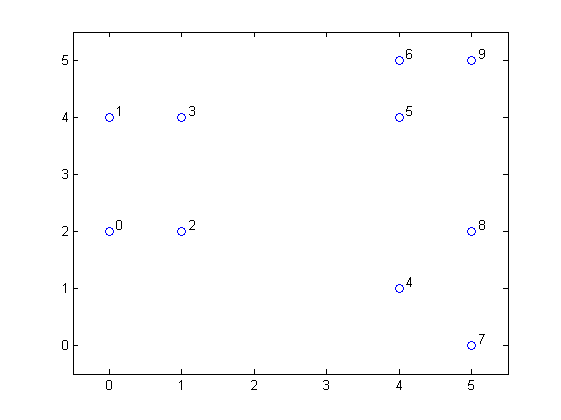
\includegraphics[bb=0 0 561 420,scale=0.37]{tsp_prob.png}
\label{fig:tsp_prob}} &
\subfigure[Subtours from the initial solution to the \ac{TSP} example]{
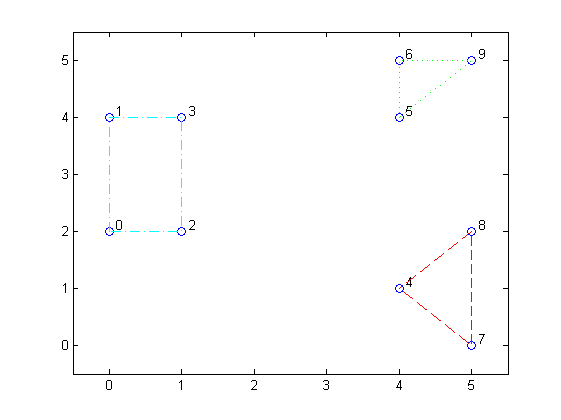
\includegraphics[bb=0 0 561 420,scale=0.37]{tsp_cuts1.png}
\label{fig:tsp_cuts1}}\\
\subfigure[Subtour from a later solution to the \ac{TSP} example]{
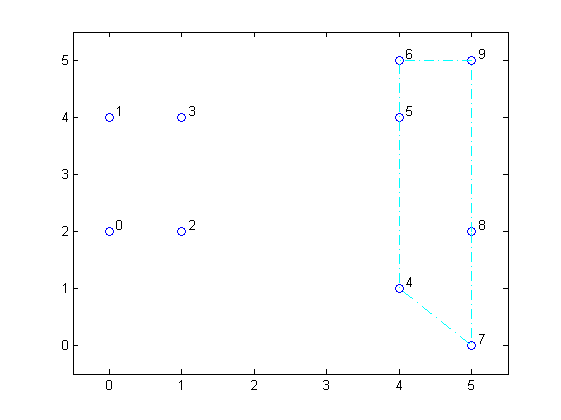
\includegraphics[bb=0 0 561 420,scale=0.37]{tsp_cuts2.png}
\label{fig:tsp_cuts2}} &
\subfigure[Final solution to the \ac{TSP} example]{
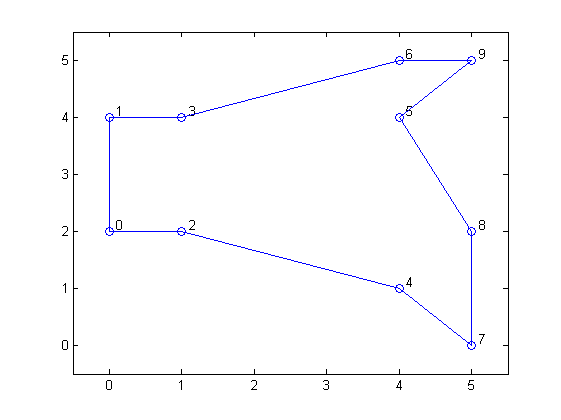
\includegraphics[bb=0 0 561 420,scale=0.37]{tsp_soln.png}
\label{fig:tsp_soln}}
\end{tabular}
\end{raggedright}
\caption{Cuts from an example \ac{TSP}} \label{fig:tsp}
\end{figure}

\begin{comment}
\subsection{Customised Cut Generation for the Wedding Planner problem} \label{sbs:wed_cuts}
\end{comment}